\documentclass[aspectratio=169]{beamer}

% ==== Theme & basic look ====
\usetheme{Madrid}
\usecolortheme{seahorse}
\setbeamertemplate{navigation symbols}{}
\setbeamertemplate{footline}[frame number]

% Packages for mathematics  
\usepackage{amsmath}  
\usepackage{mathtools}
\usepackage{amsfonts}  
\usepackage{amssymb}  
\usepackage{graphicx}
\usepackage{xcolor}
\usepackage{CJKutf8}
\usepackage{enumerate} % for enumerate[(1.)] style labels

% Support for \Tilde macro used throughout
\providecommand{\Tilde}[1]{\tilde{#1}}
\providecommand{\proofname}{Proof}
\newenvironment<>{proofs}[1][\proofname]{%
    \par
    \def\insertproofname{#1.}%
    \usebeamertemplate{proof begin}#2}
  {\usebeamertemplate{proof end}}
\makeatother

\newtheorem{remark}{Remark}

% Math shorthand and vector symbols
\newcommand{\grad}{\nabla}
\newcommand{\EE}{\mathbb{E}}
\newcommand{\dd}{\mathrm{d}}
\newcommand{\kbT}{k_B T}
\newcommand{\vx}{\mathbf{x}}
\newcommand{\vz}{\mathbf{z}}
\newcommand{\KL}{\operatorname{KL}}
\newcommand{\ELBO}{\text{ELBO}}
\DeclareMathOperator{\sg}{sg}

% ====== Shortcuts ======
\newcommand{\E}{\mathbb{E}}
\newcommand{\N}{\mathcal{N}}
\newcommand{\R}{\mathbb{R}}
\newcommand{\given}{\,|\,}

% Bold vector/time-indexed variables
\newcommand{\vxz}{\mathbf{x}}
\newcommand{\vzt}{\mathbf{z}}
\newcommand{\vtheta}{\boldsymbol{\theta}}
\newcommand{\vphi}{\boldsymbol{\phi}}
\newcommand{\veps}{\boldsymbol{\epsilon}}

% Title page details:   
\title[Understanding VAE]{Understanding Variational Autoencoders from a mathematical view}  
\author{Pipi Hu}  
\institute[BIMSA]{Beijing Institute of Mathematical Sciences and Applications}  
\date{\today}  

\pgfdeclareimage[width=2cm]{logo}{../figures/logo.png}
\logo{\pgfuseimage{logo}}

\setbeamertemplate{navigation symbols}{}
\AtBeginSection[]  
{  
    \begin{frame}<beamer>{Outline}         
        \tableofcontents[currentsection]  
    \end{frame}  
}  
  
\AtBeginSubsection[]  
{  
    \begin{frame}<beamer>{Outline}         
        \tableofcontents[currentsection,currentsubsection]  
    \end{frame}  
}  

\begin{document}  
  
% Title slide  
\begin{frame}  
  \titlepage  
\end{frame}  

\begin{frame}{Feynman's words}
\centering
    What I cannot create, I do not understand.
\end{frame}
  
% Presentation slides  

\section{Introduction: The Problem of Generative Modeling}

\begin{frame}{The Low-Dimensional Manifold Hypothesis}
\textbf{Key observation:} Natural images lie on a low-dimensional manifold, not in the full high-dimensional space.

\begin{itemize}
    \item \textbf{Full space:} $1024 \times 1024 \times 3 = 3,145,728$ dimensions
    \item \textbf{Actual manifold:} Much lower dimensional (often $< 100$ dimensions)
    \item Most of the high-dimensional space is empty or contains unrealistic images
\end{itemize}

\vspace{0.5em}
\textbf{Central question:} How can we embed these features into a compact latent space?

\begin{itemize}
    \item Capture the essential structure of the data
    \item Enable efficient representation and generation
    \item Learn meaningful features for downstream tasks
\end{itemize}
\end{frame}

\begin{frame}{Autoencoders: A Direct Approach}
\textbf{Basic idea:} Use an encoder-decoder architecture to learn compact representations

\begin{center}
\textbf{Autoencoder (AE) Architecture}
\end{center}

\begin{itemize}
    \item \textbf{Encoder:} $x \to z$ (compression)
    \item \textbf{Decoder:} $z \to \hat{x}$ (reconstruction)
    \item \textbf{Objective:} Minimize reconstruction error $\|x - \hat{x}\|^2$
\end{itemize}

\vspace{0.5em}
\textcolor{red}{\textbf{Problem:} Interpretation problems in the latent space}

\begin{columns}
\begin{column}{0.4\textwidth}
\begin{center}
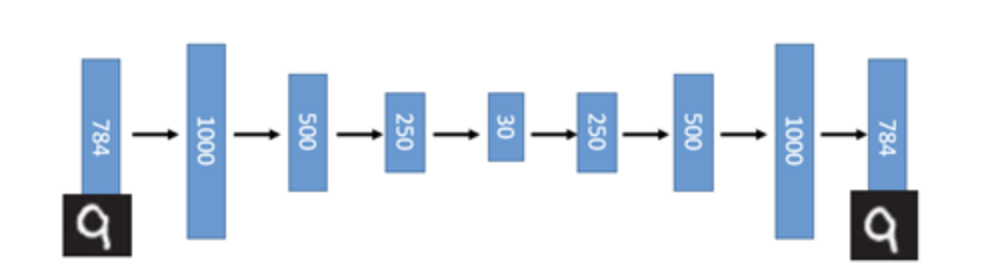
\includegraphics[width=\textwidth]{../figures/vae1.png}
\end{center}
\end{column}
\begin{column}{0.25\textwidth}
\begin{center}
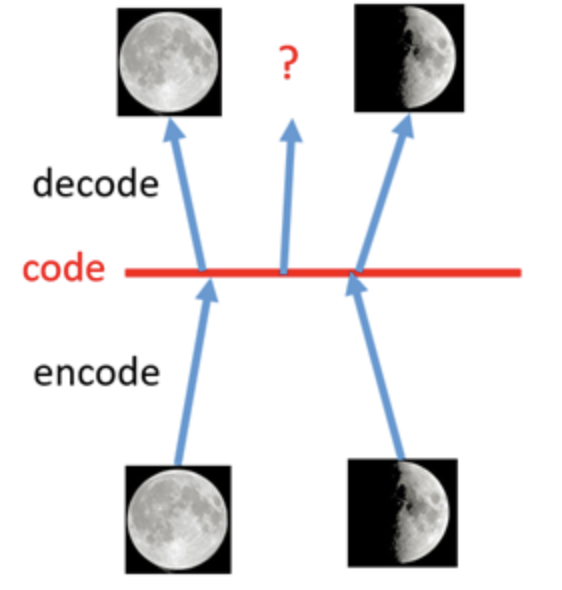
\includegraphics[width=\textwidth]{../figures/vae2.png}
\end{center}
\end{column}
\end{columns}

\end{frame}

\begin{frame}{From Deterministic to Probabilistic: Variational Autoencoders}
\textbf{Key insight:} Model encoder and decoder as \textcolor{blue}{random variables}

\begin{itemize}
    \item \textbf{Encoder:} $q_\phi(z|x)$ - maps data variable $x$ to latent variable $z$
    \item \textbf{Decoder:} $p_\theta(x|z)$ - reconstructs data from latent variable
    \item \textbf{Prior:} $p(z)$ - regularizes the latent space
\end{itemize}

\vspace{0.5em}
\textbf{Benefits:}
\begin{itemize}
    \item \textcolor{blue}{Natural interpolation} in the latent space
    \item Smooth transitions between data points
    \item Well-structured, continuous latent representation
\end{itemize}

\begin{columns}
\begin{column}{0.2\textwidth}
\begin{center}
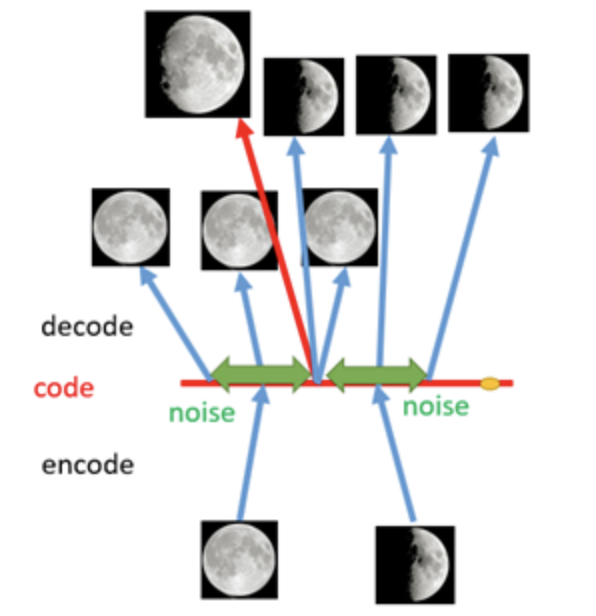
\includegraphics[width=\textwidth]{../figures/vae3.png}
\end{center}
\end{column}
\begin{column}{0.2\textwidth}
\begin{center}
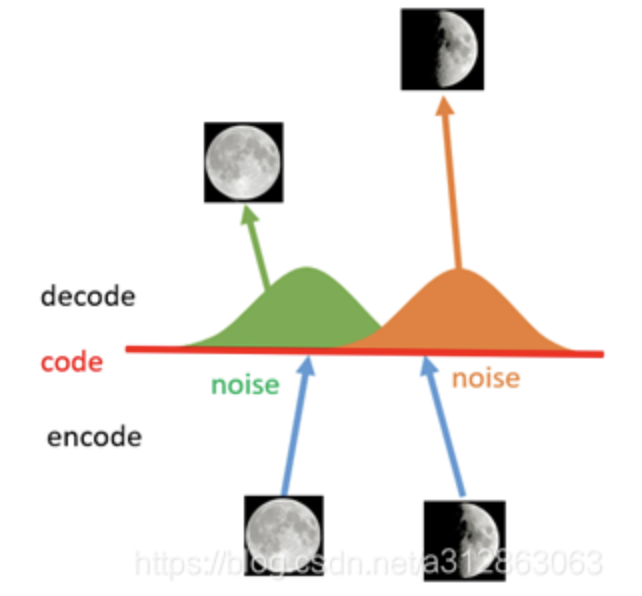
\includegraphics[width=\textwidth]{../figures/vae4.png}
\end{center}
\end{column}
\end{columns}
\end{frame}

\section{Variational Inference: The Foundation}

\begin{frame}{Latent Variable Generative Models}

\textbf{Goal.} Learn a probabilistic model that can:
\begin{itemize}
  \item Assign high probability to data: $x \sim p_{\text{data}}(x)$,
  \item Generate realistic samples,
  item Provide useful latent representations $z$.
\end{itemize}

\medskip

\textbf{Latent variable model.}
\begin{align*}
p_\theta(x,z) &= p_\theta(x \mid z)\,p(z), \\
p_\theta(x)   &= \int p_\theta(x,z)\,dz
              = \int p_\theta(x\mid z)p(z)\,dz.
\end{align*}

\textbf{Maximum likelihood objective.}
\[
\theta^* = \arg\max_\theta \mathbb{E}_{x\sim p_{\text{data}}}[\log p_\theta(x)].
\]

In practice, the expectation is replaced by the empirical average over the dataset.
\end{frame}

% ===================== Frame 2 =====================
\begin{frame}{Why the Posterior is a Problem?}

We would like to optimize the log-likelihood
\[
\log p_\theta(x) = \log \int p_\theta(x,z)\,dz.
\]

Its gradient (assuming we can interchange $\nabla$ and $\int$):
\begin{align*}
\nabla_\theta \log p_\theta(x)
&= \frac{1}{p_\theta(x)} \int \nabla_\theta p_\theta(x,z)\,dz \\
&= \int \frac{p_\theta(x,z)}{p_\theta(x)} \nabla_\theta \log p_\theta(x,z)\,dz \\
&= \mathbb{E}_{p_\theta(z\mid x)}\big[\nabla_\theta \log p_\theta(x,z)\big].
\end{align*}

\textbf{Key issue:} this expectation is taken under the \emph{posterior}
\[
p_\theta(z\mid x) = \frac{p_\theta(x,z)}{p_\theta(x)},
\]
which is typically intractable in deep models: no closed form, difficult to sample from directly.
\end{frame}

% ===================== Frame 3 =====================
\begin{frame}{Variational Inference and the ELBO (Pointwise in \textit{x})}

Idea: introduce a tractable \emph{approximate posterior} $q_\phi(z\mid x)$ and derive a lower bound on $\log p_\theta(x)$. Rewrite:
\vspace{-1em}
\begin{align*}
\log p_\theta(x)
&= \log \int p_\theta(x,z)\,dz \\
&= \log \int q_\phi(z\mid x)\,\frac{p_\theta(x,z)}{q_\phi(z\mid x)}\,dz \\
&= \log \mathbb{E}_{q_\phi(z\mid x)}
     \left[\frac{p_\theta(x,z)}{q_\phi(z\mid x)}\right].
\end{align*}

Apply Jensen's inequality (log is concave, so that $\E_p[\log X] \le \log \E_p[X]$):
\begin{align*}
\log p_\theta(x)
&\ge \mathbb{E}_{q_\phi(z\mid x)}
    \left[\log \frac{p_\theta(x,z)}{q_\phi(z\mid x)}\right]
:= \mathcal{L}(\theta,\phi; x).
\end{align*}

$\mathcal{L}(\theta,\phi;x)$ is the \textbf{Evidence Lower Bound} (ELBO).
We maximize it w.r.t.\ both $\theta$ and $\phi$.
\end{frame}

\begin{frame}{What is the gap?}

Start from the KL divergence between $q_\phi(z\mid x)$ and the true posterior $p_\theta(z\mid x)$:
\begin{align*}
\mathrm{KL}\big(q_\phi(z\mid x)\,\|\,p_\theta(z\mid x)\big)
&= \mathbb{E}_{q_\phi(z\mid x)}
   \left[\log \frac{q_\phi(z\mid x)}{p_\theta(z\mid x)}\right] \\[4pt]
&= \mathbb{E}_{q_\phi(z\mid x)}
   \left[\log q_\phi(z\mid x) - \log p_\theta(z\mid x)\right].
\end{align*}

Use Bayes' rule $p_\theta(z\mid x) = \dfrac{p_\theta(x,z)}{p_\theta(x)}$,
\begin{align*}
\Rightarrow\quad
\mathrm{KL}&=\mathbb{E}_{q_\phi(z\mid x)}
\left[\log q_\phi(z\mid x) - \log p_\theta(x,z) + \log p_\theta(x)\right].
\end{align*}

Separate the terms (note $\log p_\theta(x)$ does not depend on $z$):
\begin{align*}
\mathrm{KL}
&= \mathbb{E}_{q_\phi}[\log q_\phi(z\mid x) - \log p_\theta(x,z)]
   + \log p_\theta(x).
\end{align*}

Define the ELBO
\[
\mathcal{L}(\theta,\phi;x)
:= \mathbb{E}_{q_\phi(z\mid x)}[\log p_\theta(x,z) - \log q_\phi(z\mid x)],
\]
so that
\[
\log p_\theta(x)
= \mathcal{L}(\theta,\phi;x)
 + \mathrm{KL}\big(q_\phi(z\mid x)\,\|\,p_\theta(z\mid x)\big).
\]
\end{frame}

\begin{frame}{Summarize VAE from the generative perspective}
We have $p_{\text{data}}(x)$ and we want to learn a model $p_\theta(x)$ that can generate realistic samples from the easily sampled latent variable $z$.
\begin{itemize}
    \item We can use the maximum likelihood objective to learn the model $p_\theta(x)$.
    \[
      \nabla_\theta \log p_\theta(x) = \mathbb{E}_{p_\theta(z|x)}[\nabla_\theta \log p_\theta(x|z)]
    \]
    \item However, the gradient is intractable because the integral is over the conditional distribution $p_\theta(z|x)$ and we do not know the posterior $p_\theta(z|x)$\\
    $\rightarrow$ We replaced the posterior $p_\theta(z|x)$ with a neural network $q_\phi(z|x)$.
    \item Compute the KL divergence between $q_\phi(z|x)$ and $p_\theta(z|x)$ gives the gap:
    \[
      \mathrm{KL}(q_\phi(z|x) \| p_\theta(z|x)) = \log p_\theta(x) - \ELBO(x; \theta, \phi)
    \]
\end{itemize}

\begin{remark}
    Why did we not directly optimize $p_\theta(x)$?
\end{remark}
\end{frame}

% ===================== Frame 4 =====================
\begin{frame}{Two Views of the ELBO}

\textbf{1. Joint-form ELBO and true posterior gap.}
\begin{align*}
\mathcal{L}(\theta,\phi;x)
&= \mathbb{E}_{q_\phi(z\mid x)}[\log p_\theta(x,z) - \log q_\phi(z\mid x)], \\
\log p_\theta(x)
&= \mathcal{L}(\theta,\phi;x)
 + \mathrm{KL}\big(q_\phi(z\mid x)\,\|\,p_\theta(z\mid x)\big). 
\end{align*}

Thus for fixed $\theta$:
\[
\max_\phi \mathcal{L}(\theta,\phi;x)
\;\Longleftrightarrow\;
\min_\phi \mathrm{KL}\big(q_\phi(z\mid x)\,\|\,p_\theta(z\mid x)\big).
\]

\medskip

\textbf{2. Reconstruction--regularization form.}

Using $p_\theta(x,z)=p_\theta(x\mid z)p(z)$:
\begin{align*}
\mathcal{L}(\theta,\phi;x)
&= \mathbb{E}_{q_\phi(z\mid x)}[\log p_\theta(x\mid z)]
   - \mathrm{KL}\big(q_\phi(z\mid x)\,\|\,p(z)\big).
\end{align*}

\begin{itemize}
  \item First term: \textbf{reconstruction} (log-likelihood under decoder).
  \item Second term: \textbf{regularization} toward prior $p(z)$.
\end{itemize}
\end{frame}



% ===================== Frame 5 =====================
\begin{frame}{The VAE Architecture}

We parameterize both the generative model and the approximate posterior with neural nets.

\medskip

\textbf{Prior over latents.}
\[
p(z) = \mathcal{N}(0, I).
\]

\textbf{Decoder (generative model).}
\[
p_\theta(x\mid z)
\]
\begin{itemize}
  \item Example (continuous): 
    $p_\theta(x\mid z) = \mathcal{N}(\mu_\theta(z), \sigma^2 I)$.
  \item Example (binary): 
    $p_\theta(x\mid z) = \text{Bernoulli}(\mathrm{sigmoid}(f_\theta(z)))$.
\end{itemize}

\textbf{Encoder (approximate posterior).}
\[
q_\phi(z\mid x) = \mathcal{N}\big(\mu_\phi(x), \mathrm{diag}(\sigma^2_\phi(x))\big),
\]
where $\mu_\phi(x)$ and $\log \sigma_\phi^2(x)$ are outputs of a neural network.

\medskip

\textbf{Training objective (per-sample).}
\[
\mathcal{L}(\theta,\phi;x)
= \mathbb{E}_{q_\phi(z\mid x)}[\log p_\theta(x\mid z)]
  - \mathrm{KL}\big(q_\phi(z\mid x)\,\|\,p(z)\big).
\]
\end{frame}

% ===================== Frame 6 =====================
\begin{frame}{Reparameterization Trick}

To optimize the ELBO with SGD, we need gradients through the expectation
\[
\mathbb{E}_{q_\phi(z\mid x)}[\log p_\theta(x\mid z)].
\]

Directly sampling $z \sim q_\phi(z\mid x)$ makes the gradient w.r.t.\ $\phi$ hard to propagate.

\medskip

\textbf{Reparameterization trick:}
\begin{align*}
z &\sim q_\phi(z\mid x)
 = \mathcal{N}\big(\mu_\phi(x), \mathrm{diag}(\sigma_\phi^2(x))\big) \\
\Longrightarrow\quad
z &= \mu_\phi(x) + \sigma_\phi(x) \odot \epsilon, \\
\epsilon &\sim \mathcal{N}(0,I).
\end{align*}

Now the expectation becomes
\[
\mathbb{E}_{\epsilon\sim\mathcal{N}(0,I)}\big[\log p_\theta(x\mid 
\mu_\phi(x)+\sigma_\phi(x)\odot\epsilon)\big],
\]
which is differentiable w.r.t.\ both $\theta$ and $\phi$ using standard backprop.
\end{frame}

% ===================== Frame 7 =====================
\begin{frame}{Dataset Objective and Training}

\textbf{Population objective:}
\[
\max_{\theta,\phi} \;\; 
\mathbb{E}_{x\sim p_{\text{data}}}\big[\mathcal{L}(\theta,\phi;x)\big].
\]

Approximate with empirical average over dataset $\{x_i\}_{i=1}^N$:
\[
\max_{\theta,\phi} \;\; 
\frac{1}{N} \sum_{i=1}^N \mathcal{L}(\theta,\phi;x_i).
\]

\textbf{Mini-batch SGD:}
\begin{itemize}
  \item Sample a mini-batch $\{x_i\}_{i\in \mathcal{B}}$,
  \item For each $x_i$, sample $\epsilon^{(i)}\sim\mathcal{N}(0,I)$,
  \item Compute $z^{(i)} = \mu_\phi(x_i) + \sigma_\phi(x_i)\odot \epsilon^{(i)}$,
  \item Estimate
  \[
  \widehat{\mathcal{L}} = \frac{1}{|\mathcal{B}|}
    \sum_{i\in\mathcal{B}}\left[
      \log p_\theta(x_i\mid z^{(i)})
      - \mathrm{KL}\big(q_\phi(z\mid x_i)\,\|\,p(z)\big)
    \right],
  \]
  \item Update $(\theta,\phi)$ by ascending the gradient of $\widehat{\mathcal{L}}$.
\end{itemize}
\end{frame}

% ===================== Frame 8 =====================
\begin{frame}{Interpretations and Summary}

\textbf{1. Approximate Bayesian inference.}
\begin{itemize}
  \item ELBO decomposition:
  \[
  \log p_\theta(x)
  = \mathcal{L}(\theta,\phi;x)
    + \mathrm{KL}\big(q_\phi(z\mid x)\,\|\,p_\theta(z\mid x)\big).
  \]
  \item Maximizing ELBO $\Rightarrow$ 
    approximate maximum likelihood \emph{and}
    make $q_\phi(z\mid x)$ close to the true posterior.
\end{itemize}

\textbf{2. Rate--distortion / information bottleneck view.}
\begin{itemize}
  \item Reconstruction term: fidelity to data.
  \item KL$(q_\phi(z\mid x)\,\|\,p(z))$: ``rate'' / complexity of the code $z$.
\end{itemize}

\textbf{3. VAE in one sentence.}

A VAE is a latent-variable generative model trained by maximizing a variational lower bound on log-likelihood, with:
\begin{itemize}
  \item a decoder $p_\theta(x\mid z)$ (generator),
  \item an encoder $q_\phi(z\mid x)$ (amortized approximate posterior),
  \item and the reparameterization trick for low-variance gradients.
\end{itemize}
\end{frame}

\begin{frame}{Analytical KL Divergence}
For Gaussian distributions, the KL divergence has a closed form:
\begin{equation}
\KL(\mathcal{N}(\mu, \sigma^2) \| \mathcal{N}(0, I)) = \frac{1}{2} \sum_{j=1}^J (\mu_j^2 + \sigma_j^2 - \log \sigma_j^2 - 1)
\end{equation}

where $J$ is the dimension of the latent space.

\textbf{Interpretation:}
\begin{itemize}
    \item $\mu_j^2$: Penalizes large mean values
    \item $\sigma_j^2 - \log \sigma_j^2 - 1$: Encourages $\sigma_j \approx 1$
    \item Total effect: Regularizes latent space to be close to standard Gaussian
\end{itemize}

\textbf{Benefits:}
\begin{itemize}
    \item No sampling required for KL term
    \item Stable gradients
    \item Interpretable regularization
\end{itemize}
\end{frame}

\begin{frame}{Simplified Loss: Unit Variance Case}
Setting $\sigma_{\text{encoder}} = 1$ and $\sigma_{\text{decoder}} = 1$:

\textbf{Encoder:} $q_\phi(z|x) = \mathcal{N}(\mu_\phi(x), I)$

\textbf{Decoder:} $p_\theta(x|z) = \mathcal{N}(\mu_\theta(z), I)$

\textbf{Simplified KL term:}
\begin{equation}
\KL(q_\phi(z|x) \| p(z)) = \frac{1}{2} \|\mu_\phi(x)\|^2
\end{equation}
(since $\sigma_j = 1$ for all $j$, we have $\sigma_j^2 - \log \sigma_j^2 - 1 = 0$)

\textbf{Simplified reconstruction term:}
\begin{equation}
\EE_{q_\phi(z|x)}[\log p_\theta(x|z)] = -\frac{1}{2} \EE_{q_\phi(z|x)}[\|x - \mu_\theta(z)\|^2] + \text{const}
\end{equation}

\textbf{Total loss:}
\begin{equation}
\mathcal{L}(\theta, \phi) = \frac{1}{2} \EE_{q_\phi(z|x)}[\|x - \mu_\theta(z)\|^2] + \frac{1}{2} \|\mu_\phi(x)\|^2
\end{equation}

\textbf{Interpretation:}
\begin{itemize}
    \item First term: Reconstruction error (MSE)
    \item Second term: Regularization on encoder mean
\end{itemize}
\end{frame}

\section{VAE Variants and Extensions}

\begin{frame}{$\beta$-VAE: Controlling the Regularization}
\textbf{Motivation:} Balance between reconstruction and regularization

\textbf{$\beta$-VAE objective:}
\begin{equation}
\mathcal{L}(\theta, \phi) = \EE_{q_\phi(z|x)}[\log p_\theta(x|z)] - \beta \KL(q_\phi(z|x) \| p(z))
\end{equation}

\textbf{Effect of $\beta$:}
\begin{itemize}
    \item $\beta > 1$: Stronger regularization $\Rightarrow$ Better disentanglement
    \item $\beta < 1$: Weaker regularization $\Rightarrow$ Better reconstruction
    \item $\beta = 1$: Standard VAE
\end{itemize}

\textbf{Disentanglement:} $\beta$-VAE encourages learning of independent latent factors
\end{frame}

\begin{frame}{VQ-VAE: Vector Quantized VAE}
\textbf{Key idea:} Use discrete latent representations instead of continuous

\textbf{Architecture:}
\begin{itemize}
    \item Encoder: $z_e = E(x)$ (continuous)
    \item Quantization: $z_q = \text{Quantize}(z_e)$ (discrete)
    \item Decoder: $\hat{x} = D(z_q)$
\end{itemize}

\textbf{Quantization process:}
\begin{equation}
z_q = \arg\min_{k} \|z_e - e_k\|^2
\end{equation}
where $\{e_k\}_{k=1}^K$ are learnable codebook vectors.

\textbf{Benefits:}
\begin{itemize}
    \item Discrete representations (useful for language, etc.)
    \item Better compression
    \item Enables autoregressive modeling in latent space
\end{itemize}
\end{frame}

\begin{frame}{VQ-VAE Training}
\textbf{Challenge:} Quantization is non-differentiable

\textbf{Solution:} Straight-through estimator
\begin{equation}
\frac{\partial \mathcal{L}}{\partial z_e} = \frac{\partial \mathcal{L}}{\partial z_q}
\end{equation}

\textbf{Training objective:}
\begin{equation}
\mathcal{L} = \log p(x|z_q) + \|\sg(z_e) - e_k\|^2 + \beta\|z_e - \sg(e_k)\|^2
\end{equation}

where $\sg(\cdot)$ is stop-gradient operator.

\textbf{Components:}
\begin{itemize}
    \item Reconstruction loss: $\log p(x|z_q)$
    \item Codebook loss: $\|\sg(z_e) - e_k\|^2$ (updates codebook)
    \item Commitment loss: $\beta\|z_e - \sg(e_k)\|^2$ (encourages encoder to commit)
\end{itemize}
\end{frame}

\begin{frame}{WAE: Wasserstein Autoencoder}
\textbf{Motivation:} Replace KL divergence with Wasserstein distance

\textbf{WAE objective:}
\begin{equation}
\mathcal{L} = \EE_{p(x)} \EE_{q_\phi(z|x)} [c(x, D(z))] + \lambda \mathcal{D}(q_\phi(z), p(z))
\end{equation}

where:
\begin{itemize}
    \item $c(x, D(z))$: Reconstruction cost
    \item $\mathcal{D}(q_\phi(z), p(z))$: Distance between aggregated posterior and prior
    \item $\lambda$: Regularization weight
\end{itemize}

\textbf{Benefits:}
\begin{itemize}
    \item More flexible than KL divergence
    \item Better mode coverage
    \item Can use different distance metrics
\end{itemize}
\end{frame}

\begin{frame}{VAE-GAN: Combining VAE and GAN}
\textbf{Idea:} Use GAN discriminator to improve VAE reconstruction quality

\textbf{Architecture:}
\begin{itemize}
    \item VAE encoder-decoder: $x \to z \to \hat{x}$
    \item GAN discriminator: Distinguishes real vs reconstructed samples
    \item Generator: VAE decoder
\end{itemize}

\textbf{Training objective:}
\begin{equation}
\mathcal{L} = \mathcal{L}_{\text{VAE}} + \lambda \mathcal{L}_{\text{GAN}}
\end{equation}

where:
\begin{itemize}
    \item $\mathcal{L}_{\text{VAE}}$: Standard VAE loss
    \item $\mathcal{L}_{\text{GAN}}$: Adversarial loss for discriminator
\end{itemize}

\textbf{Benefits:}
\begin{itemize}
    \item Better sample quality than VAE alone
    \item Maintains inference capabilities
\end{itemize}
\end{frame}

\section{Advanced Topics}

\begin{frame}{Hierarchical VAE}
\textbf{Motivation:} Learn hierarchical latent representations

\textbf{Architecture:}
\begin{equation}
p_\theta(x, z_1, \ldots, z_L) = p_\theta(x|z_1) \prod_{l=1}^{L-1} p_\theta(z_l|z_{l+1}) p_\theta(z_L)
\end{equation}

\textbf{Inference:}
\begin{equation}
q_\phi(z_{1:L}|x) = \prod_{l=1}^L q_\phi(z_l|z_{<l}, x)
\end{equation}

\textbf{Benefits:}
\begin{itemize}
    \item Multi-scale representations
    \item Better modeling of complex data
    \item Hierarchical generation process
\end{itemize}
\end{frame}

\begin{frame}{Conditional VAE (C-VAE)}
\textbf{Extension:} Incorporate conditioning information

\textbf{Model:}
\begin{equation}
p_\theta(x, z|c) = p_\theta(x|z, c) p(z)
\end{equation}

\textbf{Inference:}
\begin{equation}
q_\phi(z|x, c) = \mathcal{N}(z; \mu_\phi(x, c), \sigma_\phi^2(x, c))
\end{equation}

\textbf{Applications:}
\begin{itemize}
    \item Conditional generation
    \item Controlled synthesis
    \item Multi-modal learning
\end{itemize}

\textbf{Training:}
\begin{equation}
\mathcal{L} = \EE_{q_\phi(z|x,c)}[\log p_\theta(x|z,c)] - \KL(q_\phi(z|x,c) \| p(z))
\end{equation}
\end{frame}

\begin{frame}{Importance Weighted Autoencoder (IWAE)}
\textbf{Motivation:} Better approximation of log-likelihood

\textbf{IWAE objective:}
\begin{equation}
\mathcal{L}_K = \EE_{z_1, \ldots, z_K \sim q_\phi(z|x)} \left[ \log \frac{1}{K} \sum_{k=1}^K \frac{p_\theta(x, z_k)}{q_\phi(z_k|x)} \right]
\end{equation}

\textbf{Key properties:}
\begin{itemize}
    \item $\mathcal{L}_K \geq \mathcal{L}_{K-1}$ (monotonic improvement)
    \item $\lim_{K \to \infty} \mathcal{L}_K = \log p_\theta(x)$ (exact likelihood)
    \item $K=1$ recovers standard VAE
\end{itemize}

\textbf{Trade-offs:}
\begin{itemize}
    \item Better approximation with larger $K$
    \item Higher computational cost
    \item More complex gradients
\end{itemize}
\end{frame}

\section{Practical Considerations}

\begin{frame}{Common Issues and Solutions}
\textbf{Posterior collapse:}
\begin{itemize}
    \item \textbf{Symptom:} $q_\phi(z|x) \approx p(z)$ (no information in latent)
    \item \textbf{Causes:} Strong decoder, weak encoder
    \item \textbf{Solutions:} KL annealing, free bits, stronger encoder
\end{itemize}

\textbf{Blurry reconstructions:}
\begin{itemize}
    \item \textbf{Cause:} Gaussian decoder assumption
    \item \textbf{Solutions:} VAE-GAN, better decoder architectures
\end{itemize}

\textbf{Mode collapse:}
\begin{itemize}
    \item \textbf{Symptom:} Limited diversity in generated samples
    \item \textbf{Solutions:} Better regularization, architectural improvements
\end{itemize}
\end{frame}

\begin{frame}{Evaluation Metrics}
\textbf{Reconstruction quality:}
\begin{itemize}
    \item MSE, SSIM, FID (Fréchet Inception Distance)
    \item Perceptual losses
\end{itemize}

\textbf{Generation quality:}
\begin{itemize}
    \item FID, IS (Inception Score)
    \item Human evaluation
\end{itemize}

\textbf{Representation quality:}
\begin{itemize}
    \item Disentanglement metrics ($\beta$-VAE metric, MIG)
    \item Downstream task performance
    \item Interpolation smoothness
\end{itemize}
\end{frame}

\section{Conclusion}

\begin{frame}{Summary}
\textbf{Key contributions of VAE:}
\begin{itemize}
    \item Scalable variational inference for latent variable models
    \item End-to-end training with reparameterization trick
    \item Foundation for many generative models
\end{itemize}

\textbf{VAE variants address:}
\begin{itemize}
    \item Disentanglement ($\beta$-VAE)
    \item Discrete representations (VQ-VAE)
    \item Sample quality (VAE-GAN, WAE)
    \item Hierarchical modeling (HVAE)
\end{itemize}

\textbf{Impact:}
\begin{itemize}
    \item Influenced modern generative models
    \item Enabled practical latent variable modeling
    \item Foundation for many applications
\end{itemize}
\end{frame}

\begin{frame}{Questions}
If you are interested in the questions, please feel free to write an email to me {\color{red}(\href{mailto:hpp@bimsa.cn}{hpp@bimsa.cn})} with your comments. 
\begin{enumerate}[(1.)]
    \item How does the choice of prior $p(z)$ affect VAE performance? What are the trade-offs between different priors?
    \item Can you derive the gradient of the ELBO with respect to the encoder parameters $\phi$? How does the reparameterization trick make this tractable?
    \item What are the theoretical guarantees of VAE? Under what conditions does the ELBO provide a good approximation to the true log-likelihood?
    \item How would you extend VAE to handle sequential data (like in language modeling)? What are the key challenges?
\end{enumerate}
\end{frame}

% Thank you slide  
\begin{frame}{Welcome inputs}  
  \centering  
  Any comments?
  \\[2em]
  Welcome your inputs!  
\end{frame}  
  
\end{document}
